% =============================================================================
% Lumbar L1-L5 Vertebral Body Segmentation -- Term Project (Image Processing)
%
% Compile on Overleaf:  upload the zip, hit Recompile.
% Compile locally:      pdflatex presentation.tex   (twice for TOC)
%
% Notes for compatibility:
%   * Uses the built-in Beamer "Madrid" theme -- no external themes needed.
%   * No listings, no minted, no fancy fonts -- avoids the most common
%     Overleaf compilation failures.
%   * Only stable TikZ libraries (arrows.meta, positioning).
% =============================================================================
\documentclass[aspectratio=169,11pt]{beamer}

\usetheme{Madrid}
\usecolortheme{seahorse}
\setbeamertemplate{navigation symbols}{}
\setbeamertemplate{caption}[numbered]
\setbeamercovered{transparent}

\usepackage[utf8]{inputenc}
\usepackage[T1]{fontenc}
\usepackage{lmodern}
\usepackage{graphicx}
\usepackage{booktabs}
\usepackage{amsmath}
\usepackage{amssymb}
\usepackage{xcolor}
\usepackage{tikz}
\usetikzlibrary{arrows.meta, positioning}

% --- color palette matching the app ---
\definecolor{l1red}{RGB}{220,38,38}
\definecolor{l2green}{RGB}{34,197,94}
\definecolor{l3blue}{RGB}{59,130,246}
\definecolor{l4orange}{RGB}{249,115,22}
\definecolor{l5purple}{RGB}{168,85,247}
\definecolor{accent}{RGB}{0,90,160}

\graphicspath{{figures/}}

% --- title block ---
\title[L1--L5 Segmentation]{Automated Lumbar Vertebral Body Segmentation}
\subtitle{An End-to-End ML and Image Processing Pipeline}
\author{Varun Dasoju}
\institute[Image Processing]{Term Project --- Image Processing}
\date{\today}

% =============================================================================
\begin{document}

\begin{frame}[plain]
  \titlepage
\end{frame}

\begin{frame}{Outline}
  \tableofcontents
\end{frame}

% =============================================================================
\section{Motivation}
% =============================================================================

\begin{frame}{Why Segment Lumbar Vertebrae?}
  \textbf{Clinical relevance.} Voxel-level delineation of L1--L5 vertebral
  bodies is the foundation for:
  \begin{itemize}
    \item Spinal stenosis grading
    \item Vertebral height and bone-quality measurement
    \item Pre-surgical planning, screw trajectories
    \item Quantitative bone densitometry from MRI
  \end{itemize}
  \vspace{0.6em}
  \textbf{Bottleneck:} manual delineation is slow ($\sim$30 min per case)
  and inter-observer variability is high.
  \vspace{0.6em}
  \textbf{Goal:} a fully-automated, anatomically-valid pipeline driven from
  a single sagittal T1 FLAIR scan, with an interactive desktop app for
  inspection and export.
\end{frame}

% =============================================================================
\section{Pipeline Overview}
% =============================================================================

\begin{frame}{End-to-End Pipeline}
  \centering
  \begin{tikzpicture}[
    node distance=0.45cm and 0.45cm,
    every node/.style={align=center, font=\scriptsize},
    box/.style={draw, rounded corners, minimum width=2.4cm, minimum height=0.9cm,
                fill=accent!10, draw=accent, line width=0.6pt},
    pp/.style={draw, rounded corners, minimum width=2.4cm, minimum height=0.9cm,
               fill=l4orange!18, draw=l4orange!90, line width=0.6pt},
    out/.style={draw, rounded corners, minimum width=2.4cm, minimum height=0.9cm,
                fill=l2green!18, draw=l2green!90, line width=0.6pt},
    arr/.style={-{Latex[length=2mm]}, line width=0.6pt}
  ]
    \node[box] (raw)   {Raw T1 FLAIR\\ NIfTI volume};
    \node[box, right=of raw] (prep) {Stage 1\\ Input prep};
    \node[box, right=of prep] (infer) {Stage 2\\ nnU-Net inference};
    \node[pp,  below=0.7cm of infer] (post) {Stage 3\\ Post-processing};
    \node[pp,  left=of post] (cc) {Largest CC\\ ($\geq 50$ voxels)};
    \node[pp,  left=of cc] (strip) {Sagittal strip\\ ($\pm 20\%$)};
    \node[out, below=0.7cm of strip] (nifti) {Cleaned NIfTI};
    \node[out, right=of nifti] (stl) {STL meshes\\ (LPS)};
    \node[out, right=of stl] (viz) {3-pane MPR\\ + Plotly 3D};

    \draw[arr] (raw) -- (prep);
    \draw[arr] (prep) -- (infer);
    \draw[arr] (infer) -- (post);
    \draw[arr] (post) -- (cc);
    \draw[arr] (cc) -- (strip);
    \draw[arr] (strip) -- (nifti);
    \draw[arr] (nifti) -- (stl);
    \draw[arr] (stl) -- (viz);
  \end{tikzpicture}

  \vspace{0.6em}
  \footnotesize
  Built on \textbf{nnU-Net v2} with a Residual-Encoder U-Net (ResEncUNet
  Large) and three deterministic, anatomically-informed post-processing
  rules.
\end{frame}

% =============================================================================
\section{Data}
% =============================================================================

\begin{frame}{Dataset and Image Characteristics}
  \begin{columns}[T,onlytextwidth]
    \column{0.55\textwidth}
    \textbf{Training set: \texttt{Dataset100\_SpineL1L5}}
    \begin{itemize}
      \item 459 sagittal T1 FLAIR MRI volumes
      \item Voxel-level expert labels for L1--L5
      \item 6-class problem: $\{0, 1, 2, 3, 4, 5\}$
      \item 5-fold cross-validation split
    \end{itemize}
    \vspace{0.5em}
    \textbf{Inference cohort:} 242 unseen T1 FLAIR cases.
    \vspace{0.5em}\\
    \textbf{Label legend:}\\[0.3em]
    \begin{tabular}{cl}
      {\color{l1red}\rule{0.8em}{0.8em}} & L1 \\
      {\color{l2green}\rule{0.8em}{0.8em}} & L2 \\
      {\color{l3blue}\rule{0.8em}{0.8em}} & L3 \\
      {\color{l4orange}\rule{0.8em}{0.8em}} & L4 \\
      {\color{l5purple}\rule{0.8em}{0.8em}} & L5 \\
    \end{tabular}

    \column{0.45\textwidth}
    \footnotesize
    \begin{tabular}{ll}
      \toprule
      \textbf{Property} & \textbf{Value} \\ \midrule
      Sequence       & Sagittal T1 FLAIR \\
      Median size    & $130 \times 448 \times 422$ \\
      Target spacing & $0.66 \times 0.63 \times 0.66$~mm \\
      Normalisation  & $z$-score \\
      File format    & NIfTI \texttt{.nii.gz} \\
      \bottomrule
    \end{tabular}
  \end{columns}
\end{frame}

\begin{frame}{Raw Input: Sagittal T1 FLAIR}
  \centering
  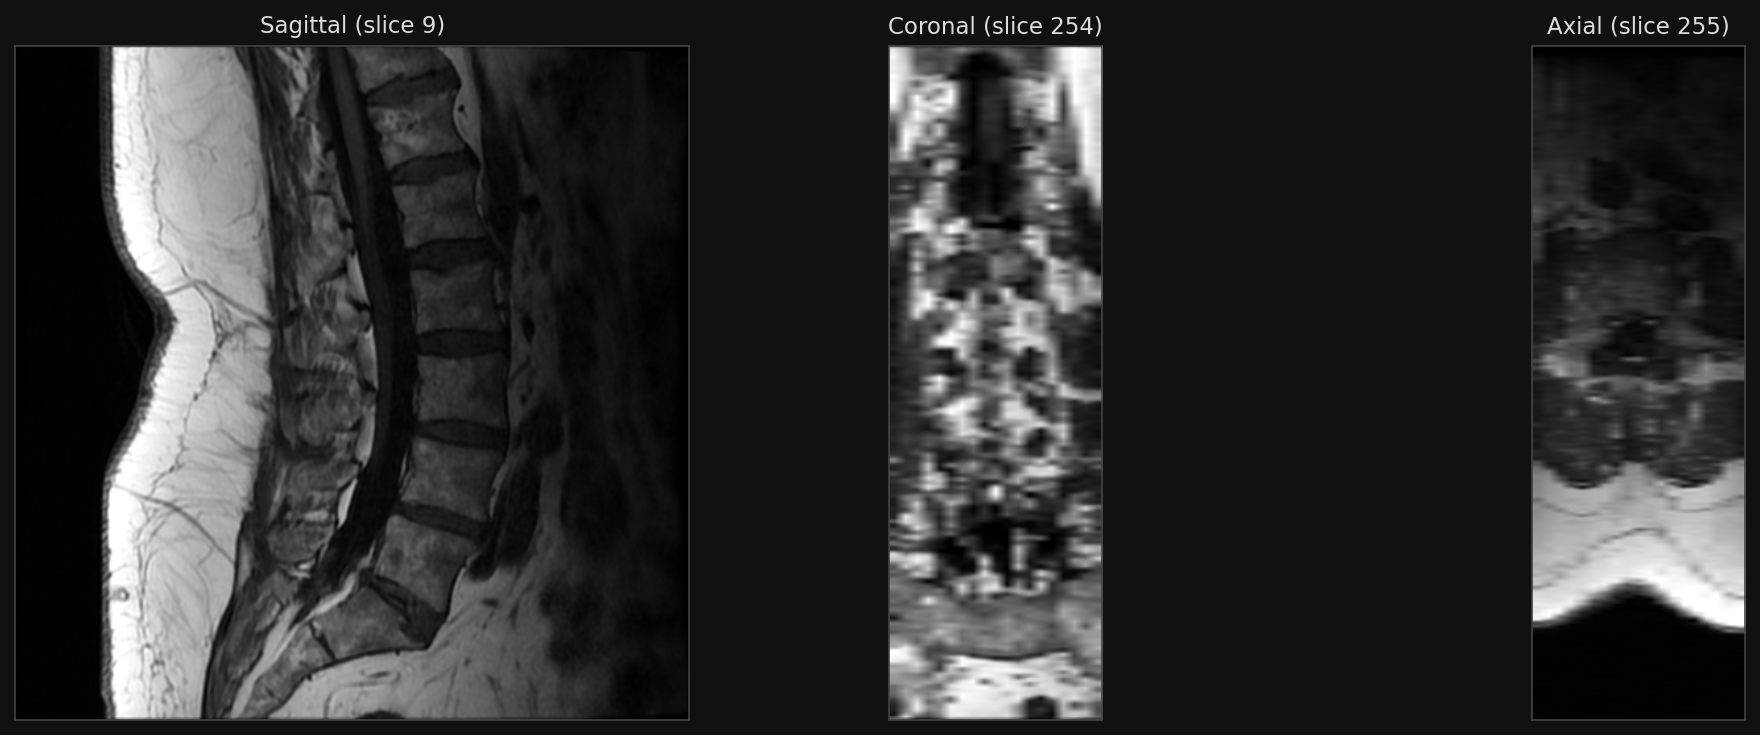
\includegraphics[width=0.95\linewidth]{mri_only.png}\\
  \vspace{0.4em}
  \footnotesize
  Mid-sagittal, mid-coronal, mid-axial slices of an unseen test volume.
  Bright cancellous bone and dark cortical rim are characteristic of T1 FLAIR.
\end{frame}

% =============================================================================
\section{Model Architecture}
% =============================================================================

\begin{frame}{nnU-Net plus Residual-Encoder U-Net (ResEncUNet Large)}
  \begin{columns}[T,onlytextwidth]
    \column{0.50\textwidth}
    \textbf{Why nnU-Net?}
    \begin{itemize}
      \item Self-configures patch size, spacing, batch
      \item State of the art on medical 3D seg
      \item Avoids manual hyper-parameter tuning
    \end{itemize}
    \vspace{0.5em}
    \textbf{Why ResEncUNet?}
    \begin{itemize}
      \item Residual blocks in encoder
      \item Better gradient flow in deep stages
      \item Up to 6 residual blocks per stage
      \item Captures both fine bone edges and large-scale spinal context
    \end{itemize}

    \column{0.50\textwidth}
    \footnotesize
    \begin{tabular}{ll}
      \toprule
      \textbf{Hyper-parameter} & \textbf{Value} \\ \midrule
      Network        & ResidualEncoderUNet \\
      Conv type      & 3D ($3\times3\times3$) \\
      Stages         & 7 \\
      Features       & 32, 64, 128, 256, 320, 320, 320 \\
      Res.\ blocks   & 1, 3, 4, 6, 6, 6, 6 \\
      Decoder convs  & 1 per stage \\
      Norm           & InstanceNorm3d \\
      Activation     & Leaky ReLU \\
      Patch size     & $80 \times 320 \times 256$ \\
      Batch size     & 2 \\
      \bottomrule
    \end{tabular}
  \end{columns}
\end{frame}

% =============================================================================
\section{Training}
% =============================================================================

\begin{frame}{Training Configuration}
  \begin{columns}[T,onlytextwidth]
    \column{0.50\textwidth}
    \textbf{Optimisation}
    \begin{itemize}
      \item SGD + Nesterov ($\mu = 0.99$)
      \item Polynomial LR decay, $\eta_0 = 10^{-2}$
      \item Loss: Dice + Cross-Entropy
      \item 1000 epochs, best-Dice checkpoint
      \item nnU-Net default augmentations \\
            (rotation, scale, mirror, gamma, elastic)
    \end{itemize}

    \column{0.50\textwidth}
    \textbf{5-Fold Cross-Validation}
    \begin{itemize}
      \item Five independent models, one per fold
      \item Per-fold checkpoint: \texttt{checkpoint\_best.pth}
      \item Inference: average softmax across folds, then \texttt{argmax}
      \item Reduces variance, smoother boundaries
    \end{itemize}
    \vspace{0.5em}
    \textbf{Inference modes (this app):}
    \begin{itemize}
      \item \textbf{1-fold} (fast, default on Mac)
      \item \textbf{5-fold ensemble} (best quality)
    \end{itemize}
  \end{columns}
\end{frame}

% =============================================================================
\section{Inference and Post-Processing}
% =============================================================================

\begin{frame}{Stage 2: Sliding-Window Ensemble Inference}
  \textbf{Command (mirrored by the app's Python API call):}
  \vspace{0.4em}

  {\footnotesize\ttfamily
  \noindent
  nnUNetv2\_predict\\
  \hspace*{1em}-i <input\_dir> -o <output\_dir>\\
  \hspace*{1em}-d 100 -c 3d\_fullres\\
  \hspace*{1em}-tr nnUNetTrainer\\
  \hspace*{1em}-p nnUNetResEncUNetLPlans\\
  \hspace*{1em}-f 0 1 2 3 4\\
  \hspace*{1em}-chk checkpoint\_best.pth -step\_size 0.5
  }
  \vspace{0.6em}
  \begin{itemize}
    \item Sliding window with 50\% overlap (\texttt{step\_size 0.5}) for smooth boundaries.
    \item Each fold produces a 6-class softmax volume.
    \item Probability maps averaged voxel-wise; final label by \texttt{argmax}.
  \end{itemize}
\end{frame}

\begin{frame}{Why Post-Process? Failure Modes of Raw Output}
  The network sees patches, not the whole spine. So raw predictions
  occasionally contain:
  \vspace{0.4em}
  \begin{itemize}
    \item \textbf{Mirror artefacts:} contralateral blobs that look spine-like
          in patch context but lie outside the vertebral column.
    \item \textbf{Disconnected fragments:} partial-volume noise on bone edges.
    \item \textbf{Ordering violations:} swapped L2/L3 etc.\ on ambiguous boundaries.
  \end{itemize}
  \vspace{0.6em}
  \textbf{Solution:} three deterministic, anatomically-informed rules,
  applied in voxel space directly to the predicted label volume.
\end{frame}

\begin{frame}{Stage 3: Anatomical Post-Processing}
  \begin{block}{Algorithm 1 -- Anatomical post-processing}
    \footnotesize
    \begin{enumerate}
      \item \textbf{Identify axes:}
            $\text{LR} = \arg\min_{a} \text{span}(S>0,\,a)$;\\
            $\text{SI} = \arg\max_{a} \text{span}(S>0,\,a)$.
      \item \textbf{Step 1 -- sagittal strip corridor:} zero out labels
            outside
            $[\,c_{\text{LR}} - 0.20\,N_{\text{LR}},\;
                c_{\text{LR}} + 0.20\,N_{\text{LR}}\,]$
            where $c_{\text{LR}}$ is the centroid along LR.
      \item \textbf{Step 2 -- largest connected component} (26-conn.):
            for each label $\ell \in \{1,\dots,5\}$, keep only the
            largest CC; drop the entire label if size $<50$ voxels.
      \item \textbf{Step 3 -- vertical (SI) ordering:} compute SI
            centroids; remove any label whose centroid breaks the
            monotonic L1 $\to$ L5 chain.
    \end{enumerate}
  \end{block}
\end{frame}

\begin{frame}{Post-Processing in Action (mid-sagittal slice)}
  \centering
  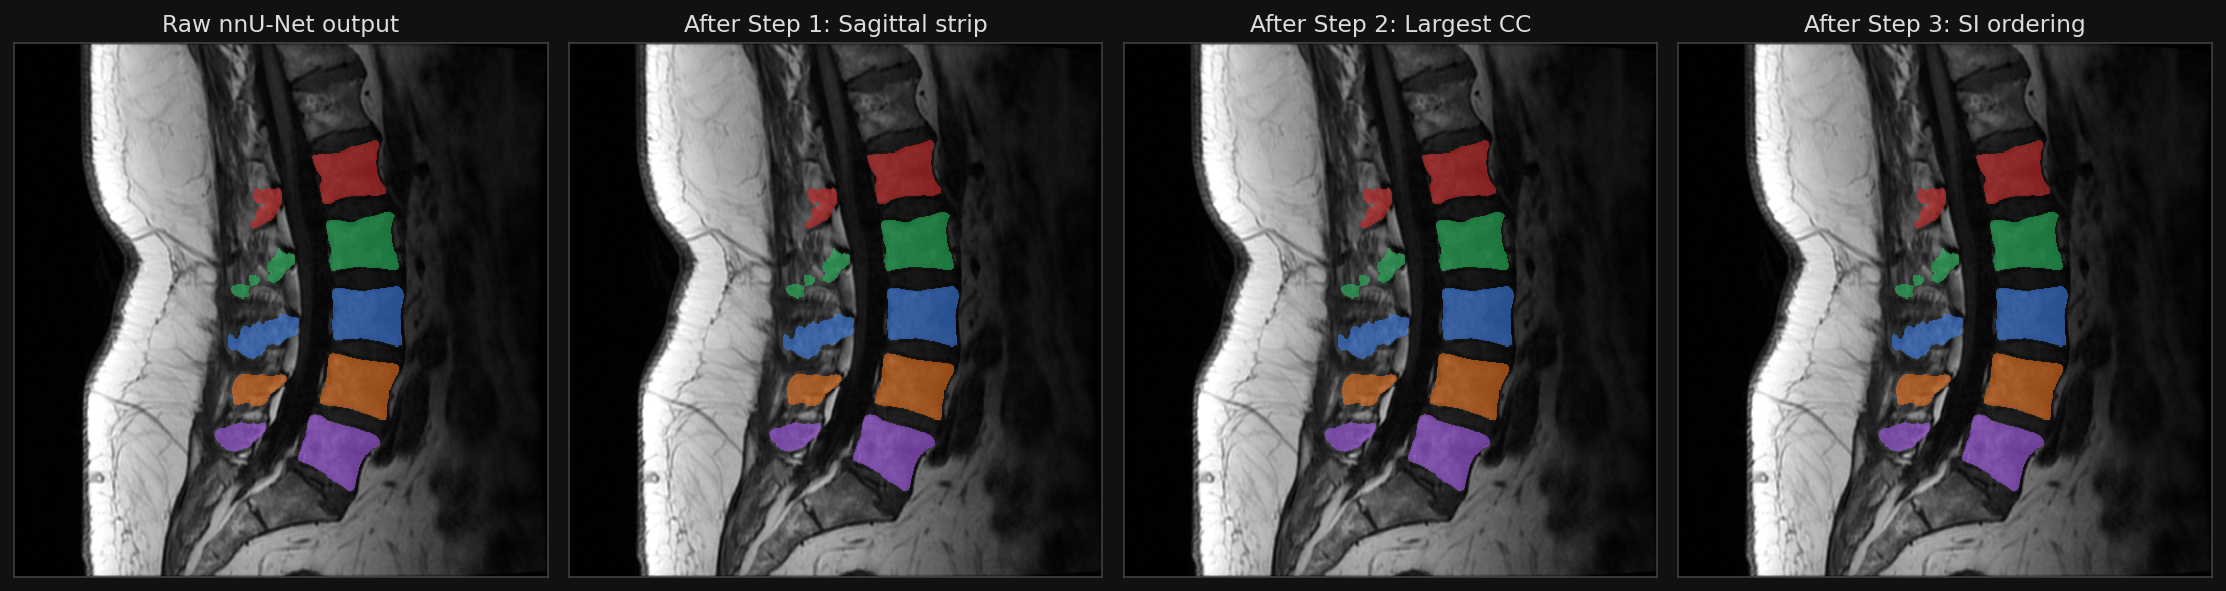
\includegraphics[width=\linewidth]{postprocess_steps.png}\\
  \vspace{0.4em}
  \footnotesize
  \begin{itemize}
    \item \textbf{Raw $\to$ Step 1:} contralateral mirror blobs eliminated.
    \item \textbf{Step 1 $\to$ Step 2:} small islands ($<50$ voxels) discarded.
    \item \textbf{Step 2 $\to$ Step 3:} ordering enforcement keeps only
          centroids consistent with L1 (sup.) $\to$ L5 (inf.) monotonicity.
  \end{itemize}
\end{frame}

% =============================================================================
\section{Mesh Extraction}
% =============================================================================

\begin{frame}{Stage 4: Voxel to Surface (Marching Cubes + Taubin)}
  \begin{columns}[T,onlytextwidth]
    \column{0.55\textwidth}
    For each retained label $\ell$:
    \begin{enumerate}
      \item Binary mask $M_\ell = (S = \ell)$
      \item 1-voxel zero pad (no boundary holes)
      \item \textbf{Marching cubes} at level 0.5
      \item Coordinate transform:\\
            voxel $\to$ NIfTI affine (RAS)\\
            $\to$ negate $X, Y$ for LPS world
      \item \textbf{Taubin smoothing} (10 iterations)\\
            volume-preserving low-pass
      \item Export STL (binary, 80-byte header)
    \end{enumerate}

    \column{0.45\textwidth}
    \centering
    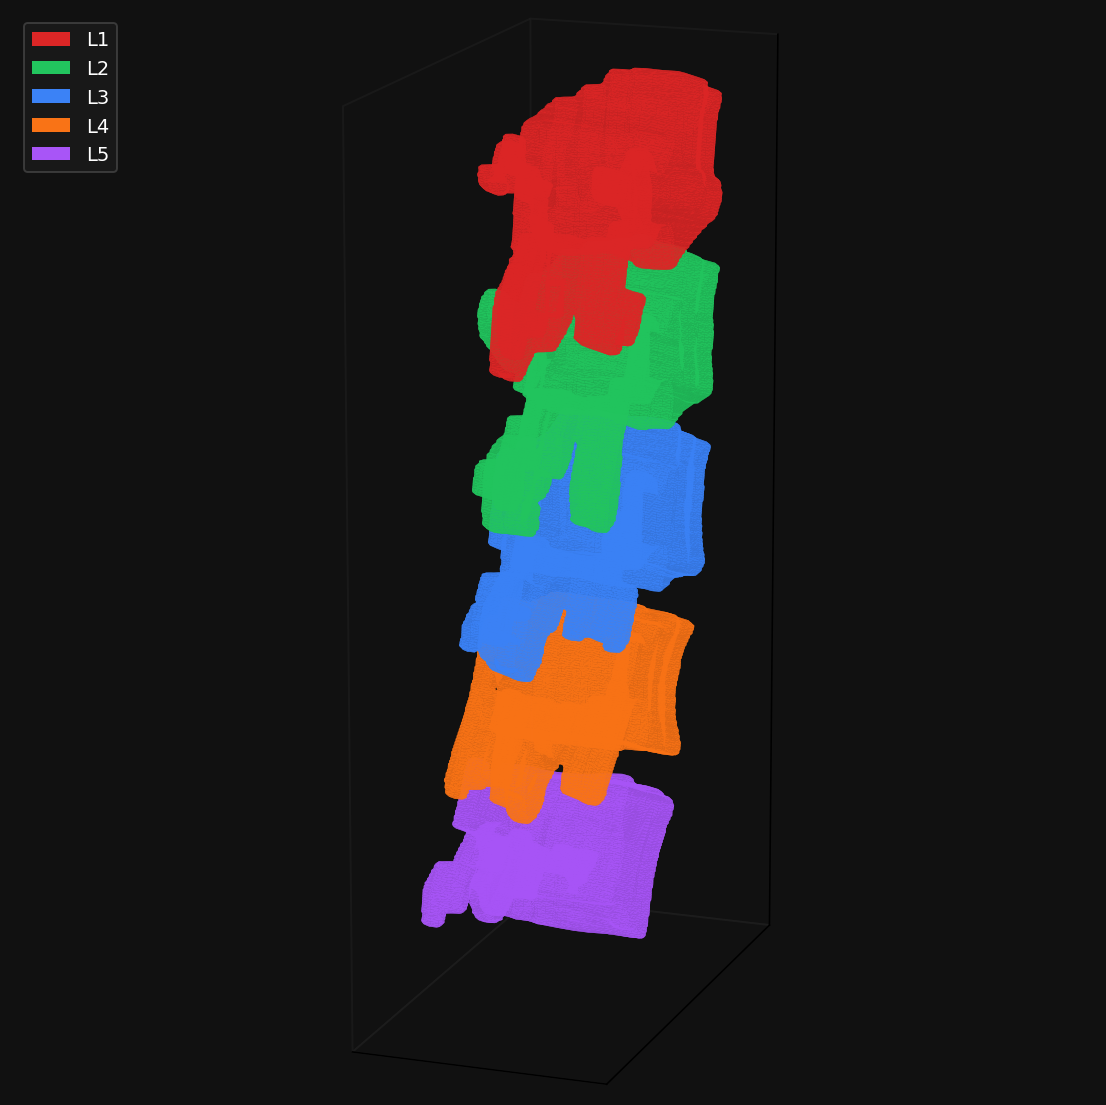
\includegraphics[width=\linewidth]{mesh_3d.png}\\
    \footnotesize
    Five smoothed surface meshes,\\ color-coded (LPS world coordinates).
  \end{columns}
\end{frame}

\begin{frame}{Taubin Smoothing in One Slide}
  \textbf{Why not Laplacian?} Iterative Laplacian smoothing shrinks the mesh.

  \vspace{0.4em}
  \textbf{Taubin:} alternate two pass-through filters with positive
  ($\lambda$) and negative ($\mu$) weights, so the magnitude transfer
  function $f(k) = (1 - \lambda k)(1 - \mu k)$ is roughly $\approx 1$
  in the low-frequency band but $<1$ at high frequencies:
  \[
    \mathbf{v}^{t+1} = (I + \mu L)(I + \lambda L)\,\mathbf{v}^{t}.
  \]
  Removes aliasing/staircase artefacts from marching cubes
  \emph{without shrinking the vertebral body}.
\end{frame}

% =============================================================================
\section{Application}
% =============================================================================

\begin{frame}{The Desktop App}
  \textbf{Stack}
  \begin{itemize}
    \item \textbf{Streamlit} for the UI
    \item \textbf{pywebview} (PyObjC + WKWebView) wraps it as a native
          macOS window --- no browser, real Dock entry
    \item \textbf{matplotlib} for the 3-pane MPR with overlay
    \item \textbf{Plotly Mesh3d} for the interactive 3D rendering
    \item \textbf{trimesh} for marching-cubes + Taubin
  \end{itemize}
  \vspace{0.4em}
  \textbf{Two launch modes}
  \begin{itemize}
    \item Double-click \texttt{launch\_spine\_seg\_app.command}
    \item CLI: \texttt{python cli.py <input.nii.gz> -o results/}
  \end{itemize}
  \vspace{0.4em}
  \textbf{File support:} single .nii / .nii.gz \emph{or} a folder of cases;
  per-file upload limit 600~MB; outputs saved to
  \texttt{./results/<case\_id>/}.
\end{frame}

\begin{frame}{App Architecture}
  \centering
  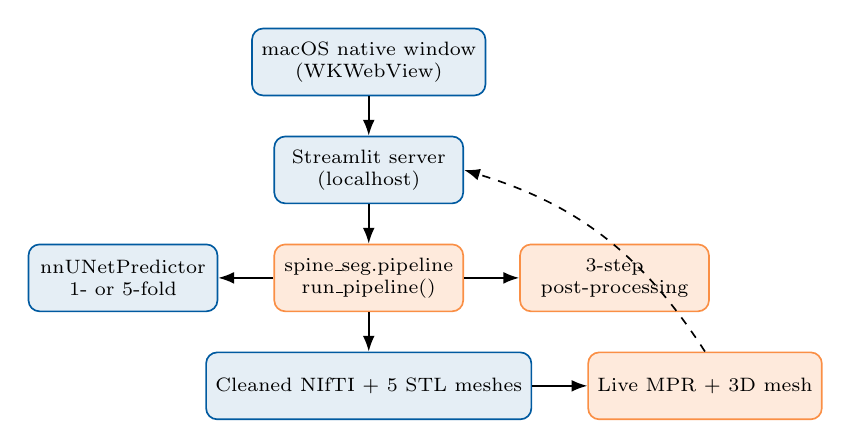
\begin{tikzpicture}[
    every node/.style={align=center, font=\scriptsize},
    box/.style={draw, rounded corners, minimum width=2.4cm, minimum height=0.85cm,
                fill=accent!10, draw=accent, line width=0.6pt},
    pp/.style={draw, rounded corners, minimum width=2.4cm, minimum height=0.85cm,
               fill=l4orange!15, draw=l4orange!80, line width=0.6pt},
    arr/.style={-{Latex[length=2mm]}, line width=0.6pt}
  ]
    \node[box] (win)  {macOS native window\\ (WKWebView)};
    \node[box, below=0.5cm of win]  (st) {Streamlit server\\ (localhost)};
    \node[pp,  below=0.5cm of st]   (pipe) {spine\_seg.pipeline\\ run\_pipeline()};
    \node[box, left=0.7cm of pipe]  (inf) {nnUNetPredictor\\ 1- or 5-fold};
    \node[pp,  right=0.7cm of pipe] (post) {3-step\\ post-processing};
    \node[box, below=0.5cm of pipe] (out) {Cleaned NIfTI + 5 STL meshes};
    \node[pp, right=0.7cm of out] (viz) {Live MPR + 3D mesh};

    \draw[arr] (win)  -- (st);
    \draw[arr] (st)   -- (pipe);
    \draw[arr] (pipe) -- (inf);
    \draw[arr] (pipe) -- (post);
    \draw[arr] (pipe) -- (out);
    \draw[arr] (out)  -- (viz);
    \draw[arr, dashed] (viz.north) to[bend right=20] (st.east);
  \end{tikzpicture}
\end{frame}

% =============================================================================
\section{Results}
% =============================================================================

\begin{frame}{Result: Multi-Planar View with Segmentation Overlay}
  \centering
  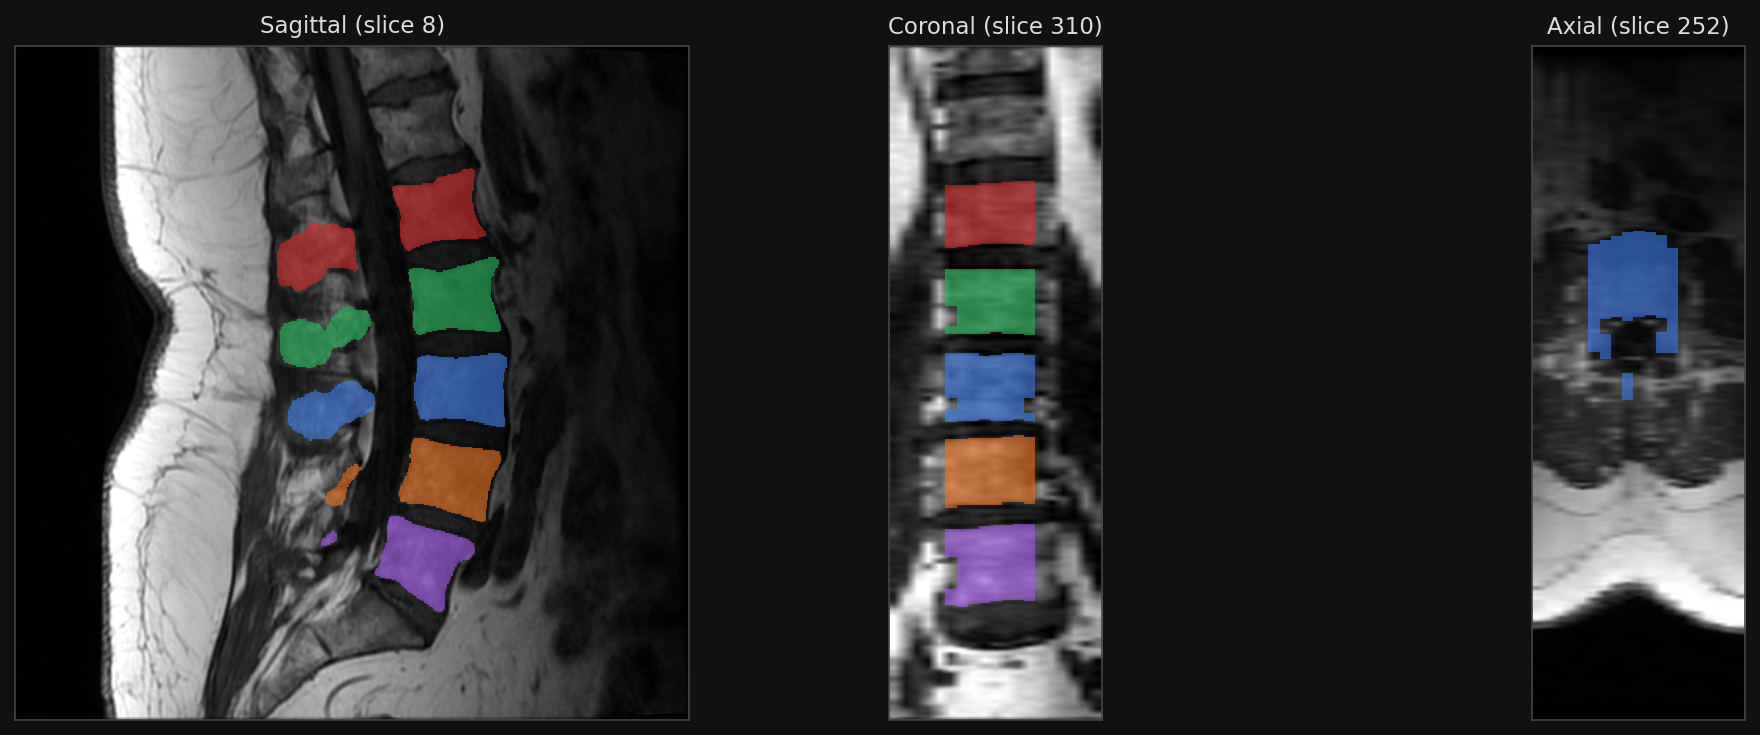
\includegraphics[width=\linewidth]{mpr_overlay.png}\\
  \vspace{0.3em}
  \footnotesize
  Same volume as before (real T1 FLAIR, never seen during training).
  Sliders in the app re-render the panels live; bilinear interpolation on
  the MRI keeps the through-plane axis readable, while
  \emph{nearest-neighbour} on the labels keeps boundaries crisp.
\end{frame}

\begin{frame}{Result: 3D Surface Reconstruction}
  \centering
  \begin{columns}[T,onlytextwidth]
    \column{0.55\textwidth}
    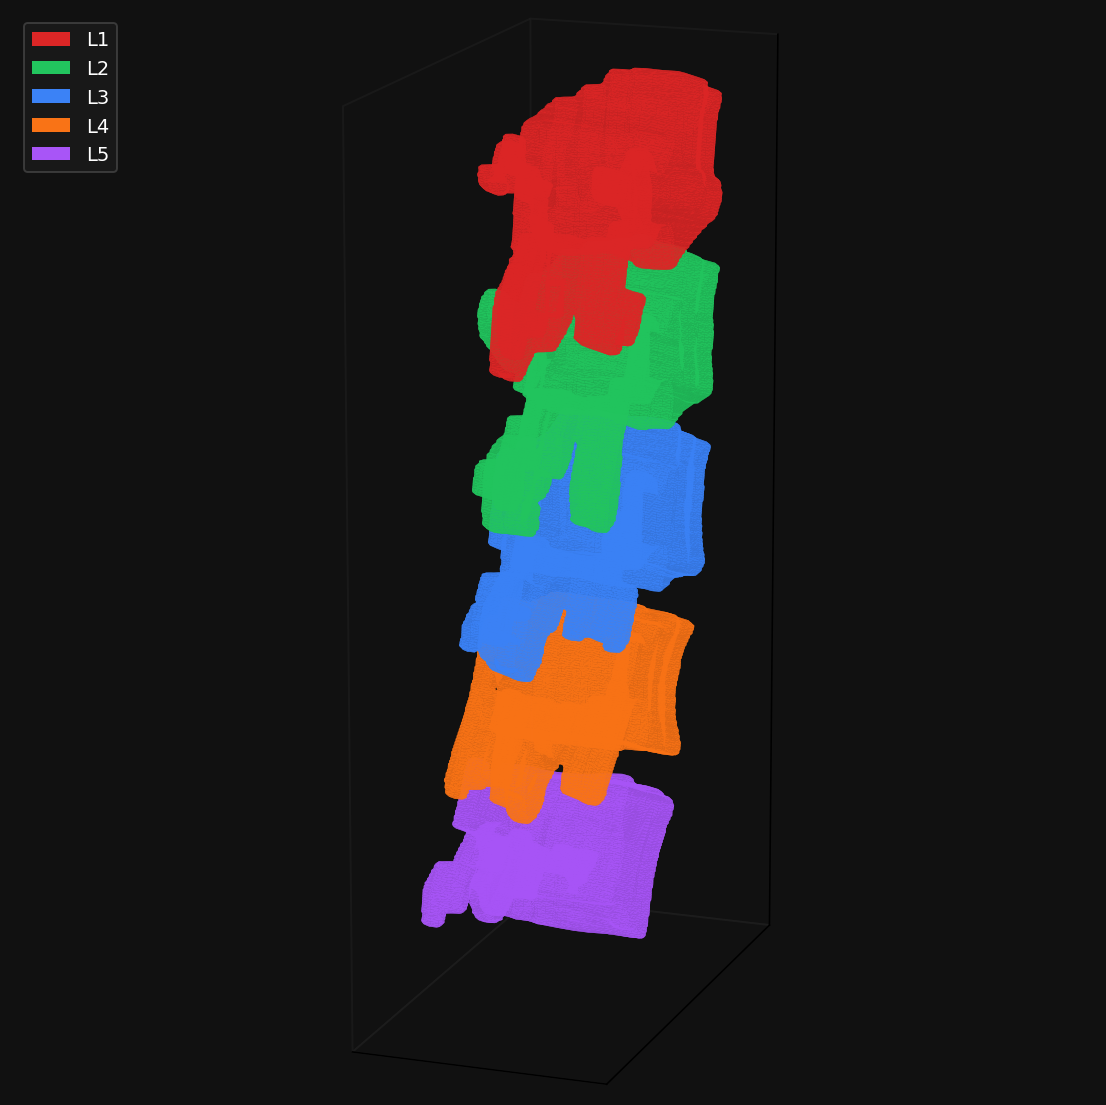
\includegraphics[width=\linewidth]{mesh_3d.png}

    \column{0.45\textwidth}
    \footnotesize
    Each surface from \textbf{marching cubes} on the cleaned label volume,
    Taubin-smoothed, transformed to LPS world coordinates.
    \\[0.6em]
    Plotly Mesh3d in the app:
    \begin{itemize}
      \item Drag to rotate, scroll to zoom
      \item Click legend to toggle individual vertebrae
      \item STLs also export cleanly into 3D Slicer
    \end{itemize}
  \end{columns}
\end{frame}

\begin{frame}{Quantitative: Per-Vertebra Voxel Counts}
  \centering
  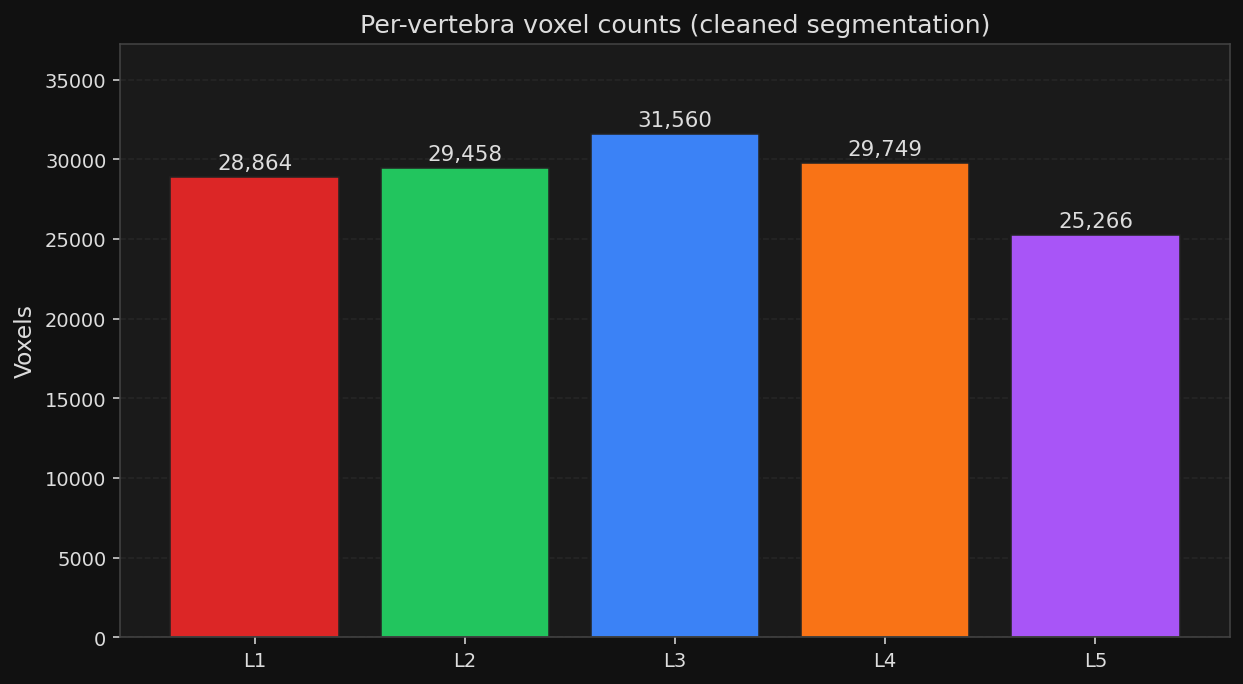
\includegraphics[width=0.92\linewidth]{voxel_counts.png}\\
  \vspace{0.3em}
  \footnotesize
  Cleaned segmentation, single test case. All five lumbar bodies were
  detected; counts decrease toward L5, matching the smaller anatomical
  extent of the lower lumbar bodies in this subject.
\end{frame}

\begin{frame}{Computational Performance (Apple M1 Max)}
  \centering
  \begin{tabular}{lll}
    \toprule
    \textbf{Mode} & \textbf{Time / case} & \textbf{Notes} \\ \midrule
    1-fold (MPS, default)         & $\sim$12~min      & interactive use \\
    5-fold ensemble (MPS)         & $\sim$50--60~min  & best quality \\
    Single fold (CPU)             & $\sim$25--35~min  & fallback \\
    Post-processing (per case)    & $<$1~s            & SciPy CC + numpy \\
    Mesh extraction (per case)    & $\sim$3--4~s      & all 5 vertebrae \\
    \bottomrule
  \end{tabular}
  \vspace{0.7em}\\
  \footnotesize
  Reference RTX 5090 numbers from the published pipeline:
  $\sim$15~s (1 fold) / $\sim$60~s (5-fold ensemble). MPS on M1 Max is
  $\sim$50$\times$ slower for this network --- acceptable for a
  single-user desktop app.
\end{frame}

% =============================================================================
\section{Limitations and Conclusion}
% =============================================================================

\begin{frame}{Limitations}
  \begin{itemize}
    \item \textbf{Modality:} model is T1-FLAIR-specific. T2 / STIR will
          produce poor segmentations until re-trained on those contrasts.
    \item \textbf{Anatomical assumption:} the SI ordering rule assumes a
          standard 5-vertebra lumbar spine. Transitional vertebrae
          (lumbarised S1, sacralised L5) can lose a label legitimately;
          inspect the kept \texttt{raw\_prediction/} for QA.
    \item \textbf{Inference latency on Apple Silicon:} the 5-fold ensemble
          is too slow ($\sim$1~h/case) for true real-time use.
          CUDA hardware collapses this to seconds.
    \item Voxel-space post-processing is robust but \emph{ignores affine
          orientation}; works because LR/SI axes are inferred from the
          labeled bounding box.
  \end{itemize}
\end{frame}

\begin{frame}{Conclusion}
  \begin{itemize}
    \item Built a complete pipeline:\\
          \emph{Raw T1 FLAIR} $\to$ \emph{nnU-Net inference} $\to$
          \emph{3-step anatomical post-processing} $\to$
          \emph{NIfTI + STL} $\to$ \emph{interactive desktop app}.
    \item Three deterministic image-processing rules (sagittal corridor,
          largest CC, SI ordering) eliminate the dominant failure modes
          of a purely data-driven model.
    \item Marching cubes + Taubin smoothing produce surface meshes that
          register correctly with the source MRI in 3D Slicer (LPS).
    \item Native-window app (Streamlit + pywebview) offers a real
          desktop-app experience on macOS with no browser.
  \end{itemize}
  \vspace{0.6em}
  \begin{center}
    \large\bfseries\color{accent}
    From a $130\times448\times422$ NIfTI to a clinical-grade segmentation
    in one click.
  \end{center}
\end{frame}

\begin{frame}[plain]
  \begin{center}
    \vspace{1.5cm}
    {\Huge\bfseries Thank You}\\[1em]
    {\large Questions?}\\[2em]
    \footnotesize\itshape
    Code: \texttt{spine\_seg\_app/}\quad
    Trained model: \texttt{nnUNet\_results/Dataset100\_SpineL1L5}
  \end{center}
\end{frame}

\end{document}
